\documentclass[10pt]{article}

\usepackage[margin=1in]{geometry}
\usepackage{times}
\usepackage{amsmath,amssymb,amsthm}
\usepackage{enumitem}
\usepackage{graphicx}
\usepackage[hidelinks]{hyperref}
\usepackage[numbers]{natbib}
\usepackage{booktabs}
\usepackage{multirow}
\usepackage[table]{xcolor}
\usepackage{caption}
\usepackage{float}
\usepackage{tikz}
\usetikzlibrary{shapes,arrows,positioning,calc}

\theoremstyle{definition}
\newtheorem{definition}{Definition}[section]

\title{Swarm Search and Rescue with Differing Scales of Autonomy}
\author{}
\date{}

\begin{document}
\maketitle

\begin{abstract}
\textcolor{red}{There are fundamentally three ways to frame this I think:}
\begin{enumerate}
    \item \textcolor{red}{Assistive systems like this are being deployed into swarm interfaces generally. This is a way to understand how giving that autonomy control to the user really works and its implications.}
    \item \textcolor{red}{The Levels of Autonomy scale concerns a ``depth'' of autonomy but not so much a ``breadth/scale'' of autonomy. This looks at the scale more than the depth}
    \item \textcolor{red}{Autonomy in defence adjacent contexts - should it be tactical, strategic, or both. When does each make sense?}
\end{enumerate}
\end{abstract}

% -----------------------------------------------------------------
\section{Introduction}\label{sec:intro}

The deployment of large numbers of robots has advanced from speculation from practice in a short time frame. Present applications of drones and similar uncrewed vehicles are increasingly requiring either large numbers of well-organised operators~\cite{ramchurn2016disaster}, or else provide early demonstrations of semi-autonomous command-and-control software~\cite{anduril2023lattice}. There is significant appetite for the incorporation of autonomy for reasons including but not limited to the impracticalities of supporting one pilot for each asset, and a desire for a single operator to maintain a complete picture of the entire operation~\cite{mod2022ukairpower}. As swarms scale further, the one-to-one or many-to-one models of human control must give way to a one-to-many paradigm, and some degree of autonomy becomes not merely desirable but unavoidable.

How that autonomy is best integrated, however, remains an open question. Autonomy is far from new; defence operations have long been organised around autonomy at different levels of a hierarchy. Auftragstaktik (mission command) requires strategic command to communicate high-level goals to subordinates and grants them latitude over low-level execution, and indeed further delegation. A similar logic can be applied to robot swarms: tactical decisions may be delegated to individual assets or sub-groups, while strategic decisions remain with a human commander. Yet it is not obvious that the best configuration places the tactical under full autonomy while leaving the strategic entirely manual. Lower-level interventions may benefit heavily from human oversight; robots still struggle with physical execution, while  autonomous planners are near-perfect at many allocation problems. Of course, higher-level decisions carry greater consequence and arguably warrant closer human control; it is natural to prefer an autonomy-at-tactical approach, however the best possible combination of autonomy levels may not be so simple. Each of these judgements also depends on operator workload and situational context. The need for interfaces and control paradigms which allow autonomy is therefore high~\cite{mod2022ukairpower}, but the question of \textit{where} in a command hierarchy that autonomy should sit, and whether this should be fixed or operator-configurable, has received little attention. Previous works have explored many forms of autonomy~\cite{nam_trust_2018}, but these have typically been treated at the level of a single decision layer.

%The recent trend in agentic design patterns provides myriad approaches to assistive tools which are deferred to by a human operator, or else proactively make suggestions to them. Such tools may provide a promising direction in human-swarm interface design~\cite{zhang2023understanding}. An additional concern is when autonomy should be employed and at what level of a decision hierarchy. Operators should be given the choice to use these tools where preferred, but it would be beneficial to understand what their experiences are, both subjectively and objectively, as the accuracy of those tools varies. Factors such as task complexity likely have significant impact on the performance of a human-autonomy team, the workload and trust of the operator, and ultimately when and where autonomous assistance is appropriate.

%Real-world deployments rarely involve a single tier of autonomous support. A drone operator managing a search-and-rescue response faces at least two interleaved decision problems: how to allocate resources to incoming missions, and how to prioritise effort within a given mission once resources are committed. Autonomous tools could assist at either level, and their reliability at each level may differ. Yet to our knowledge, no prior work has examined whether operators are more tolerant of imperfect autonomy at higher or lower levels of such a hierarchy, or how inaccuracy at one level propagates into trust at the other.



This work represents a first step toward a longer-term vision: We aim to understand how autonomy effects both user and mission when deployed at each level of a multi-layered command hierarchy, and move towards a system where each level of concern from strategic down to tactical details, can be automated to varying degrees. Finally, we propose a ``co-pilot'' that, instead of attempting to fully automate the mission, identifies where the user is most needed, and suggest to them an autonomy profile which adapts on-the-fly.

We develop a simulated search-and-rescue scenario using a heterogeneous drone swarm, and characterise how operators interact with a two-tier assistive system compared to a fully manual baseline. In a within-subjects counterbalanced design (agent-assisted vs.\ manual), we address the following research questions:
\begin{itemize}
  \item \textbf{RQ1}: Does access to the assistive system improve operator performance, and under what situational conditions is the benefit largest?
  \item \textbf{RQ2}: When the assistive system is available, do operators use it selectively---more readily under high mission complexity or low reserve depth, and less so when the situation is under control?
  \item \textbf{RQ3}: What advantage does agent-assisted allocation confer relative to manual allocation, in terms of score, asset utilisation, and mission completion time?
\end{itemize}

% -----------------------------------------------------------------
\section{Related Work}\label{sec:relatedwork}

Essential to any autonomous system is the notion of trust. Trust in this context is defined by Lee and See as ``the attitude that an agent will help achieve an individual's goals in a situation characterized by uncertainty and vulnerability''~\cite{lee2004trust}. Such qualities are abundant in swarm contexts, where the positions, motions, and goals of the robots are rife with uncertainty, and there is a significant risk of failure stemming from the attritable nature of many such assets and the high levels of risk in their environment~\cite{soorati2024enabling}. It is an important consideration, as a system which is not trusted will likely not be used by the operator, and a system which is trusted too much will be relied on without appropriate checking and oversight. A system which balances under- and over-trust is said to be well calibrated~\cite{mcdermott2019practical}.

It has been observed that once a user falls into the trap of under- or over-trust, they have a tendency to remain there unless actively coaxed back into a well-calibrated relationship~\cite{okamura_adaptive_2020}. The standard tool for this is explanations, however these are not always given due attention~\cite{naiseh_explainable_2021, wagner_explanation_2021}, and often-times users are biased in favour of action over inaction so accept suggestions readily~\cite{mosier_automation_1999}. In the domain of HSI the notion of neglect benevolence describes the observed advantage from leaving the swarm to resolve its own behaviour instead of intervening overly often~\cite{nagavalli2014neglect}, additionally supporting the notion of autonomy which manages itself under human supervision instead of constant interaction with the recommender. Equally important to explanations, then, may be a design pattern where users work in tandem with autonomous tools and can elect to deploy them selectively, with varying levels of autonomy on varying scales of a swarm or sub-swarm.

Traditionally swarm robotic systems are characterised by autonomy, however with the importance of human oversight a question arises as to what level of autonomy should be given, and how the human's actions interface with some level of autonomy. Traditional scales such as Sheridan and Verplank's LOAs are a common metric~\cite{sheridan1978human}, as well as more swarm-focussed scales of a similar form~\cite{hocraffer_meta-analysis_2017}. An important note in more developed robotic systems is that the degree of autonomy can vary at different parts of the robot's role (for example information acquisition may be more autonomous than decision-making)~\cite{onnasch_taxonomy_2021}.

An important note is that the terms ``automation'' and ``autonomy'' are often used interchangeably but are in fact different things, with the former describing well-defined processes of tasks deferred to an \textit{automated system}, and the latter describing \textit{autonomous systems} which can make ``decisions independent of human control''~\cite{lyons_humanautonomy_2021}. As we are referring to swarm robots in this work, the terms are somewhat more interchangeable, as to automate a swarm on a particular task requires the granting of some degree of autonomy (for example performing decentralised allocation, where an automated algorithm runs across robots who then autonomously resolve their tasks~\cite{delle2012methodology}). We tend to prefer the term autonomy as it is more relevant to classical swarm paradigms, but remind the reader that there can be some distinction dependent on use case.

Similar to calibrating trust, it is important that any assistive autonomous system is sufficiently performant to merit use. Human performance in the presence of such an agent is highly sensitive to the reliability and performance of that agent~\cite{rovira_effects_2007}. Some degree of imperfection is an expectation (otherwise there would be no need for a human), and humans are typically willing to tolerate occasional failure if it represents an adequate time- and effort-save. In fact, the most trusted systems are often those which sit in between `too poor to trust' and `too reliable to bother checking'~\cite{kate2018trustworthiness}.

Another important factor is the level of workload. Prior works have found that under high task load, more reliable automation increases operator performance, however under low task load, more reliable automation actually \textit{decreases} operator performance. This is likely due to the over-trust issue discussed above, and presents a difficult challenge to designers, as users may defer to the agent even when not overloaded~\cite{parasuraman_adaptive_2009}.

The level of chosen autonomy will necessarily represent a trade-off between different desirable qualities as alluded to above, and no single solution is likely to best suit every scenario~\cite{miller_delegation_nodate}. This motivates a flexible approach where the level of autonomy is not fixed, rather it can be chosen by the operator. Such flexible approaches have been explored to the extent where agents can be granted autonomy where desirable~\cite{hardin_using_nodate}, or else autonomous agents can be overridden at any level while they attempt to perform autonomously~\cite{valero-gomez_impact_2011}. So-called mixed-initiative approaches to swarm control allow a human to switch the entire swarm between manual and autonomous modes~\cite{nam_trust_2018}. To our knowledge, however, no prior work has examined the behaviour of an operator when autonomous assistance is structured into a two-tier hierarchy and the operator is free to use it selectively. Such a design allows us to ask not only whether the assistive system improves performance, but \emph{when} operators choose to engage it and what advantage that engagement confers.

We term the two structural dimensions of selective autonomy the \textbf{Depth} and \textbf{Breadth} of autonomy. \textbf{Depth} refers to how autonomous some agent is, pertaining directly to Sheridan and Verplank's LOAs~\cite{sheridan1978human}. \textbf{Breadth} refers to the scale of autonomy, whether that be an individual asset, a mission's worth of assets, or the entire reserve. The present work extends this framework by stacking two agents vertically in a hierarchy---one operating at the within-mission (tactical) level and one at the cross-mission (strategic) level---and asking how imperfection at each level is experienced by the operator.

Metrics exist to assess the difficulty of tasks in the context of swarms, such as efficiency and effectiveness, and it has been suggested that autonomy should vary depending on these~\cite{hussein_characterization_2022}. As well as the complexity of the task, a more direct assessment of cognitive complexity via operator state metrics such as EEG has been employed~\cite{abbass_augmented_2014}, and such signals could in principle inform a meta-level recommendation system.


% -----------------------------------------------------------------
\section{Scenario and Task Design}\label{sec:task}

\subsection{Operational Scenario}

We design a simulated search-and-rescue operation. The operator manages a heterogeneous reserve of autonomous assets that must be allocated to incoming rescue missions. Missions arrive at irregular intervals and consist of several individual tasks, each of which demands a particular combination of asset types to complete. The operator must decide how many and which assets to commit to each mission, balancing the need to resolve current missions quickly against holding sufficient reserve for future demand. This scenario was chosen to provide resource scarcity managed by a two-level decision structure: strategic decisions about which assets to deploy to which mission, and tactical decisions about how to prioritise effort within a mission once resources are committed.

\subsection{Asset Types}\label{sec:assets}

The reserve comprises three asset types with distinct capabilities and speeds. In the standard preset the pool is 18 Blue, 9 Red, and 3 Green drones (30 total); assets return to reserve automatically after completing their task chain.

\paragraph{Blue --- Reconnaissance Drones (18 units).}
Lightweight quadrotors equipped with a standard optical camera. Fast and rapid to redeploy. Blues perform basic visual survey, coordinate deliveries, and are the basis of most missions. They are the most abundant asset.

\paragraph{Red --- Aid Drones (9 units).}
Heavier rotary-wing platforms carrying medical supplies and provisions. Reds are necessary for any task requiring physical delivery.

\paragraph{Green --- Thermal/Specialist Units (3 units).}
More expensive platforms equipped with thermal imaging. Greens are essential for detailed area reconnaissance and for locating casualties in obscured environments; they are the rarest and slowest asset. Their scarcity is the primary driver of allocation pressure.

\subsection{Task Types}\label{sec:tasks}

There are five task types of increasing complexity and reward value (Table~\ref{tab:tasks}). They each have a specific requirement of assets to perform them (primary composition), but in some cases using additional Blue drones when specialist assets are unavailable can be an option (substitute composition).

\begin{table}[H]
\centering
\caption{Task types: primary composition and substitute. Execution times and reward values are listed in Table~\ref{tab:params}.}
\label{tab:tasks}
\small
\renewcommand{\arraystretch}{1.2}
\begin{tabular}{llll}
\toprule
\textbf{Type} & \textbf{Name} & \textbf{Primary} & \textbf{Sub.} \\
\midrule
T1 & Recce          & 1\,B             & ---           \\
T2 & Recon          & 3\,B + 1\,G      & 8\,B          \\
T3 & Minor Drop     & 1\,B + 1\,R      & 3\,B          \\
T4 & Major Drop     & 1\,B + 2\,R      & 3\,B + 1\,R   \\
T5 & Search \& Supply & 1\,R + 1\,G   & ---           \\
\bottomrule
\end{tabular}
\end{table}

\begin{itemize}[noitemsep]
  \item \textbf{T1 Recce.} A single Blue photographs an area of interest.
  \item \textbf{T2 Recon.} Detailed area survey combining optical and thermal coverage: three Blues sweep systematically while one Green provides thermal imaging, dramatically accelerating the search. Without a Green, eight Blues perform the same sweep optically but use far more assets.
  \item \textbf{T3 Minor Drop.} Supply delivery to a located casualty: one Blue identifies the precise drop point; one Red delivers aid. Without a Red, three Blues can carry a lighter cargo load.
  \item \textbf{T4 Major Drop.} Larger-scale delivery requiring heavier lift: one Blue coordinates while two Reds transport substantial payload. At least one Red is always required; the substitute replaces one Red with three Blues.
  \item \textbf{T5 Search \& Supply.} Combined casualty search and immediate triage. The Green's thermal camera locates and triages the casualty; the Red delivers medical supplies. No substitution is possible.
\end{itemize}

\subsection{Missions and Complexity}\label{sec:missions}

A mission is a bundle of tasks drawn from the five types above, the mix determined by category. Missions arrive via a Poisson process; the operator can see all active missions simultaneously. Five categories capture a gradient of severity, penalty rate, and specialist demand (Table~\ref{tab:categories}).

\begin{table}[H]
\centering
\caption{Mission categories and task composition. Penalty rates and maximum scores are listed in Table~\ref{tab:params}.}
\label{tab:categories}
\small
\renewcommand{\arraystretch}{1.2}
\begin{tabular}{lll}
\toprule
\textbf{Cat.} & \textbf{Name} & \textbf{Task mix} \\
\midrule
A & Routine       & 3--4$\times$T1, 2--3$\times$T2, 1$\times$T3           \\
B & Moderate      & T5, T4, 2$\times$T3, 2$\times$T2, 2$\times$T1          \\
C & Significant   & T5, 2$\times$T4, 2$\times$T3, 2$\times$T2, T1          \\
D & Critical      & 2$\times$T5, 2$\times$T4, 2$\times$T3, 2$\times$T2     \\
E & Mass Casualty & 3$\times$T5, 2$\times$T4, 2$\times$T3, T2, T1          \\
\bottomrule
\end{tabular}
\end{table}

\begin{itemize}[noitemsep]
  \item \textbf{Category~A (Routine).} Primarily T1 and T2 tasks with one T3; Blue and Green demand only. Fast to clear with moderate reserve drain.
  \item \textbf{Category~B (Moderate).} Includes the first mandatory T5 (Green + Red, no substitute) and one T4. Moderate Green pressure; the 8-Blue T2 substitute is feasible if Green is scarce.
  \item \textbf{Category~C (Significant).} One T5 (unavoidable Green commitment) and two T4s alongside three lighter tasks. Green scarcity begins to bite; a T5 and T4 competing for the same Green forces sequencing decisions.
  \item \textbf{Category~D (Critical).} Two T5s and two T4s. The two unavoidable Green commitments make this the primary bottleneck category; Red pressure is also high.
  \item \textbf{Category~E (Mass Casualty).} Three T5s plus two T4s; maximum pressure on all specialist assets. Likely infeasible to complete fully without a well-stocked reserve and careful Green redeployment across tasks.
\end{itemize}

The operator does not know the exact task composition of an incoming mission until it arrives. A category probability forecast is visible at all times, enabling principled hedging decisions about reserve depth\footnote{This is implemented but no longer communicated to the user clearly. It may be an necessary detail.}.

\subsection{Performance Metric}\label{sec:metric}

Performance is measured as the net score $S$ accumulated over a session of duration $T$:
\begin{equation}
S = \sum_{m \in \mathcal{M}} \left[
    \sum_{k \in \mathcal{T}_m} w_k \cdot \mathbf{1}[\text{task } k \text{ completed}]
    \;-\; r_m \cdot \bigl(\min(t^c_m, T) - t^a_m\bigr)
    \right]
\label{eq:score}
\end{equation}
where $w_k$ is the reward weight of task type $k$ (see Table~\ref{tab:params}), $r_m$ is the category-specific penalty rate, $t^a_m$ is the mission arrival time, and $t^c_m$ is the completion time (session end if not finished). Penalty scales exponentially from arrival, growing rapidly as unresolved missions accumulate; the net score therefore rewards both completing tasks and doing so quickly. Secondary measures include Green utilisation efficiency (fraction of Green asset-time on T4/T5 tasks), mean mission completion time, and reserve depth at allocation events.

% -----------------------------------------------------------------
\section{Assistive System Design}\label{sec:agents}

The assistive system comprises two tiers operating at different decision levels.

\subsection{Strategic Agent}\label{sec:strategic}

The Strategic Agent activates when the operator initiates allocation of a queued mission. It analyses the mission's task composition and the current reserve state, then presents two pre-computed strategies (Figure~\ref{fig:agent}):

\begin{itemize}[noitemsep]
  \item \textbf{Aggressive} --- commits the maximum feasible drone counts (parallel sum of all task requirements, capped by reserve), minimising expected completion time at the cost of reserve depth.
  \item \textbf{Conservative} --- favours whichever asset types are most plentiful relative to demand, using substitute compositions where specialist drones are scarce, then adds a 30\,\% top-up above the bare minimum; preserves reserve at the cost of a longer ETA.
\end{itemize}

Each strategy card displays the proposed drone counts, projected ETA, a \emph{speed score} (fraction of the minimum achievable completion time), and a \emph{reserve score} (fraction of specialist drones preserved). The operator may accept a strategy, select it and modify individual counts before deploying, or dismiss the modal and allocate manually via type-count spinners (the manual condition workflow described in Section~\ref{sec:interface}).

Accepting a strategy moves the mission to \emph{tactical-pending} state and opens the tactical planner (Section~\ref{sec:interface}) on the map window, where the operator confirms or adjusts the specific drone-to-task assignments before execution begins.

\paragraph{Error injection.} With probability $\varepsilon_S$ the displayed asset counts for one strategy are subtly corrupted: either \emph{inflated} by 2--3 units on a randomly chosen drone type (the reserve appears worse than reality) or \emph{deflated} by 2--3 units (the ETA appears optimistic because fewer drones than shown will actually execute). The true values used for deployment are unaffected; only the displayed figures mislead. Neither the error nor the condition is communicated to participants.

\subsection{Tactical Agent}\label{sec:tactical}

The Tactical Agent operates at the within-mission level, advising the operator on how to assign specific drone assets to individual tasks once a high-level allocation has been committed. It is an always-visible widget on the primary display that evaluates the current reserve state against the expected future mission load and recommends whether to \emph{preserve}, \emph{maintain}, or \emph{spend down} specialist reserve depth---informing how aggressively the operator should commit Greens to the current mission given that a Category~D or~E mission may arrive within minutes.

As with the Strategic Agent, a noise parameter $\varepsilon_T$ controls reliability. At $\varepsilon_T = 0$ the recommendation reflects the true expected value of reserve depth given the forecast; at higher $\varepsilon_T$ the forecast is perturbed before the recommendation is computed, causing the Tactical Agent to recommend postures that are systematically too conservative or too aggressive.

% -----------------------------------------------------------------
\section{Platform and Interface}\label{sec:interface}

\subsection{Interface Layout}

The platform is a browser-based simulation designed for a two-monitor setup. The \emph{primary window} (Figure~\ref{fig:primary}) runs on the main monitor and provides the command console; the \emph{map window} runs on a second monitor and provides the strategic map and tactical planner.

The primary window has three regions: (1) a \textbf{reserve bar} (top) showing live counts of available and deployed drones per type; (2) a \textbf{mission queue} (left) listing all incoming and active missions as cards, each showing category, task-type progress icons, a real-time penalty bar, accrual rate, ETA, and --- once allocated --- a collapsible drone assignment plan; and (3) an \textbf{embedded strategic map} (right) showing the hub, all mission zones, and live drone positions. Zones labelled \textit{allocate} await the operator's attention; clicking any active or tactical-pending zone opens it in the map window.

\begin{figure}[H]
  \centering
  
\includegraphics[width=\linewidth]{figs/1}
  \caption{Primary command window at the start of a session.
           \textbf{Left Panel: } Reserve of drones, and list of missions. For each mission, the set of constituent tasks is shown as well as the climbing penalty (explained below).
           \textbf{Right Panel: } Map showing each mission and the drone hub. Can be viewed at varying levels of abstraction down to showing individual asset paths.}
  \label{fig:primary}
\end{figure}

\subsection{Allocation: Manual Condition}

In the manual condition no strategy suggestions are shown. Clicking \textit{Allocate} on a mission opens a compact modal (Figure~\ref{fig:manual}) with $+$/$-$ spinners for each drone type and a live ETA computed from the greedy task schedule. An infeasible allocation (too few drones to cover even a substitute composition) displays $\infty$. Pressing \textit{Deploy} commits the counts and starts execution.

\begin{figure}[H]
  \centering
  
\includegraphics[width=0.52\linewidth]{figs/2}
  \caption{Manual allocation modal for a Category~B mission.
           The operator sets per-type counts; ETA updates live.
           Here 4\,B, 4\,R, 2\,G are committed from an 18\,B/9\,R/3\,G reserve.}
  \label{fig:manual}
\end{figure}

\subsection{Allocation: Agent-Assisted Condition}

In the agent condition, clicking \textit{Allocate} shows the Strategic Agent strategy modal (Figure~\ref{fig:agent}) with the Aggressive and Conservative cards described in Section~\ref{sec:strategic}. Selecting a strategy immediately transitions the mission to tactical-pending and opens the \textbf{tactical planner} (Figure~\ref{fig:tactical}) in the map window.

\begin{figure}[H]
  \centering
  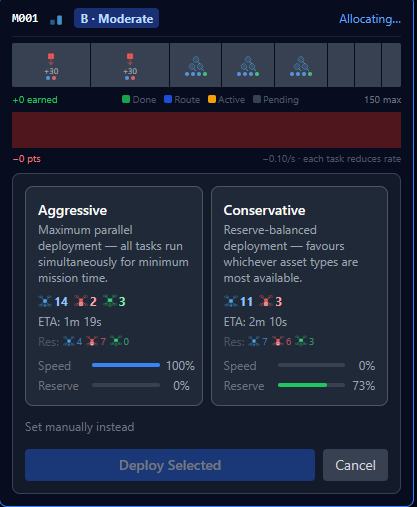
\includegraphics[width=0.52\linewidth]{figs/7}
  \caption{Strategic Agent strategy modal (agent condition) for a Category~B mission.
           }
  \label{fig:agent}
\end{figure}

The tactical planner shows the mission zone with drone icons on the boundary and dashed arrows indicating planned task assignments. The operator may drag any drone onto a task waypoint to reassign it; holding Shift while dropping \emph{chains} the drone to execute a second task after the first. Sequence numbers on the arrows indicate execution order. A \textit{Deploy} button activates once every task has at least a substitute-feasible composition; pressing it begins execution.

\begin{figure}[H]
  \centering
  
\includegraphics[width=\linewidth]{figs/3}
  \caption{Tactical planner (map window).
           Drone icons around the zone boundary.
           Task circles show type name and current drone-count progress (e.g.\ 0/1\,B\,0/1\,R for a Minor Drop).
           The right panel lists tasks with assigned drones; \textit{Deploy} activates once all tasks are feasible.}
  \label{fig:tactical}
\end{figure}

\subsection{Mid-Session State}

\begin{figure}[H]
  \centering
  
\includegraphics[width=\linewidth]{figs/4}
  \caption{Mid-session primary display.
           At the highest detail level, every asset's path is visible (this can be abstracted away). Notice on the left the penalty for each mission scales exponentially over time, incentivising faster resolution of tasks.}
  \label{fig:active}
\end{figure}

\subsection{Drone Failure and Recovery}

Approximately once per session, one deployed drone fails. The affected mission card displays a red banner naming the lost drone (Figure~\ref{fig:failure}). Clicking the mission opens the tactical planner in \emph{recovery mode} (Figure~\ref{fig:recovery}), pre-loaded with the current allocation minus the failed drone.

\begin{figure}[H]
  \centering
  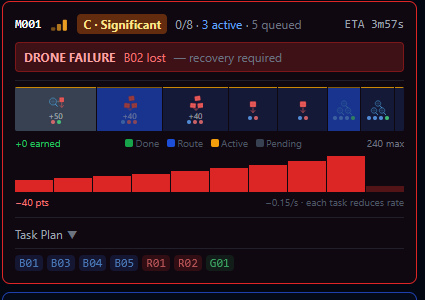
\includegraphics[width=0.6\linewidth]{figs/5}
  \caption{Drone failure notification on a Category~C mission card.
           The red banner identifies the lost drone (B02).}
  \label{fig:failure}
\end{figure}

In recovery mode, executing tasks carry amber badges and travelling tasks carry blue badges; the failed drone appears greyed-out with a red cross. A cluster of up to five reserve drones per type is anchored at the HUB corner of the zone; the operator drags reserve drones onto tasks to restore feasibility, chains them for sequential execution, or redistributes existing drones. \textit{Deploy} commits the updated plan and resumes execution.

\begin{figure}[H]
  \centering
  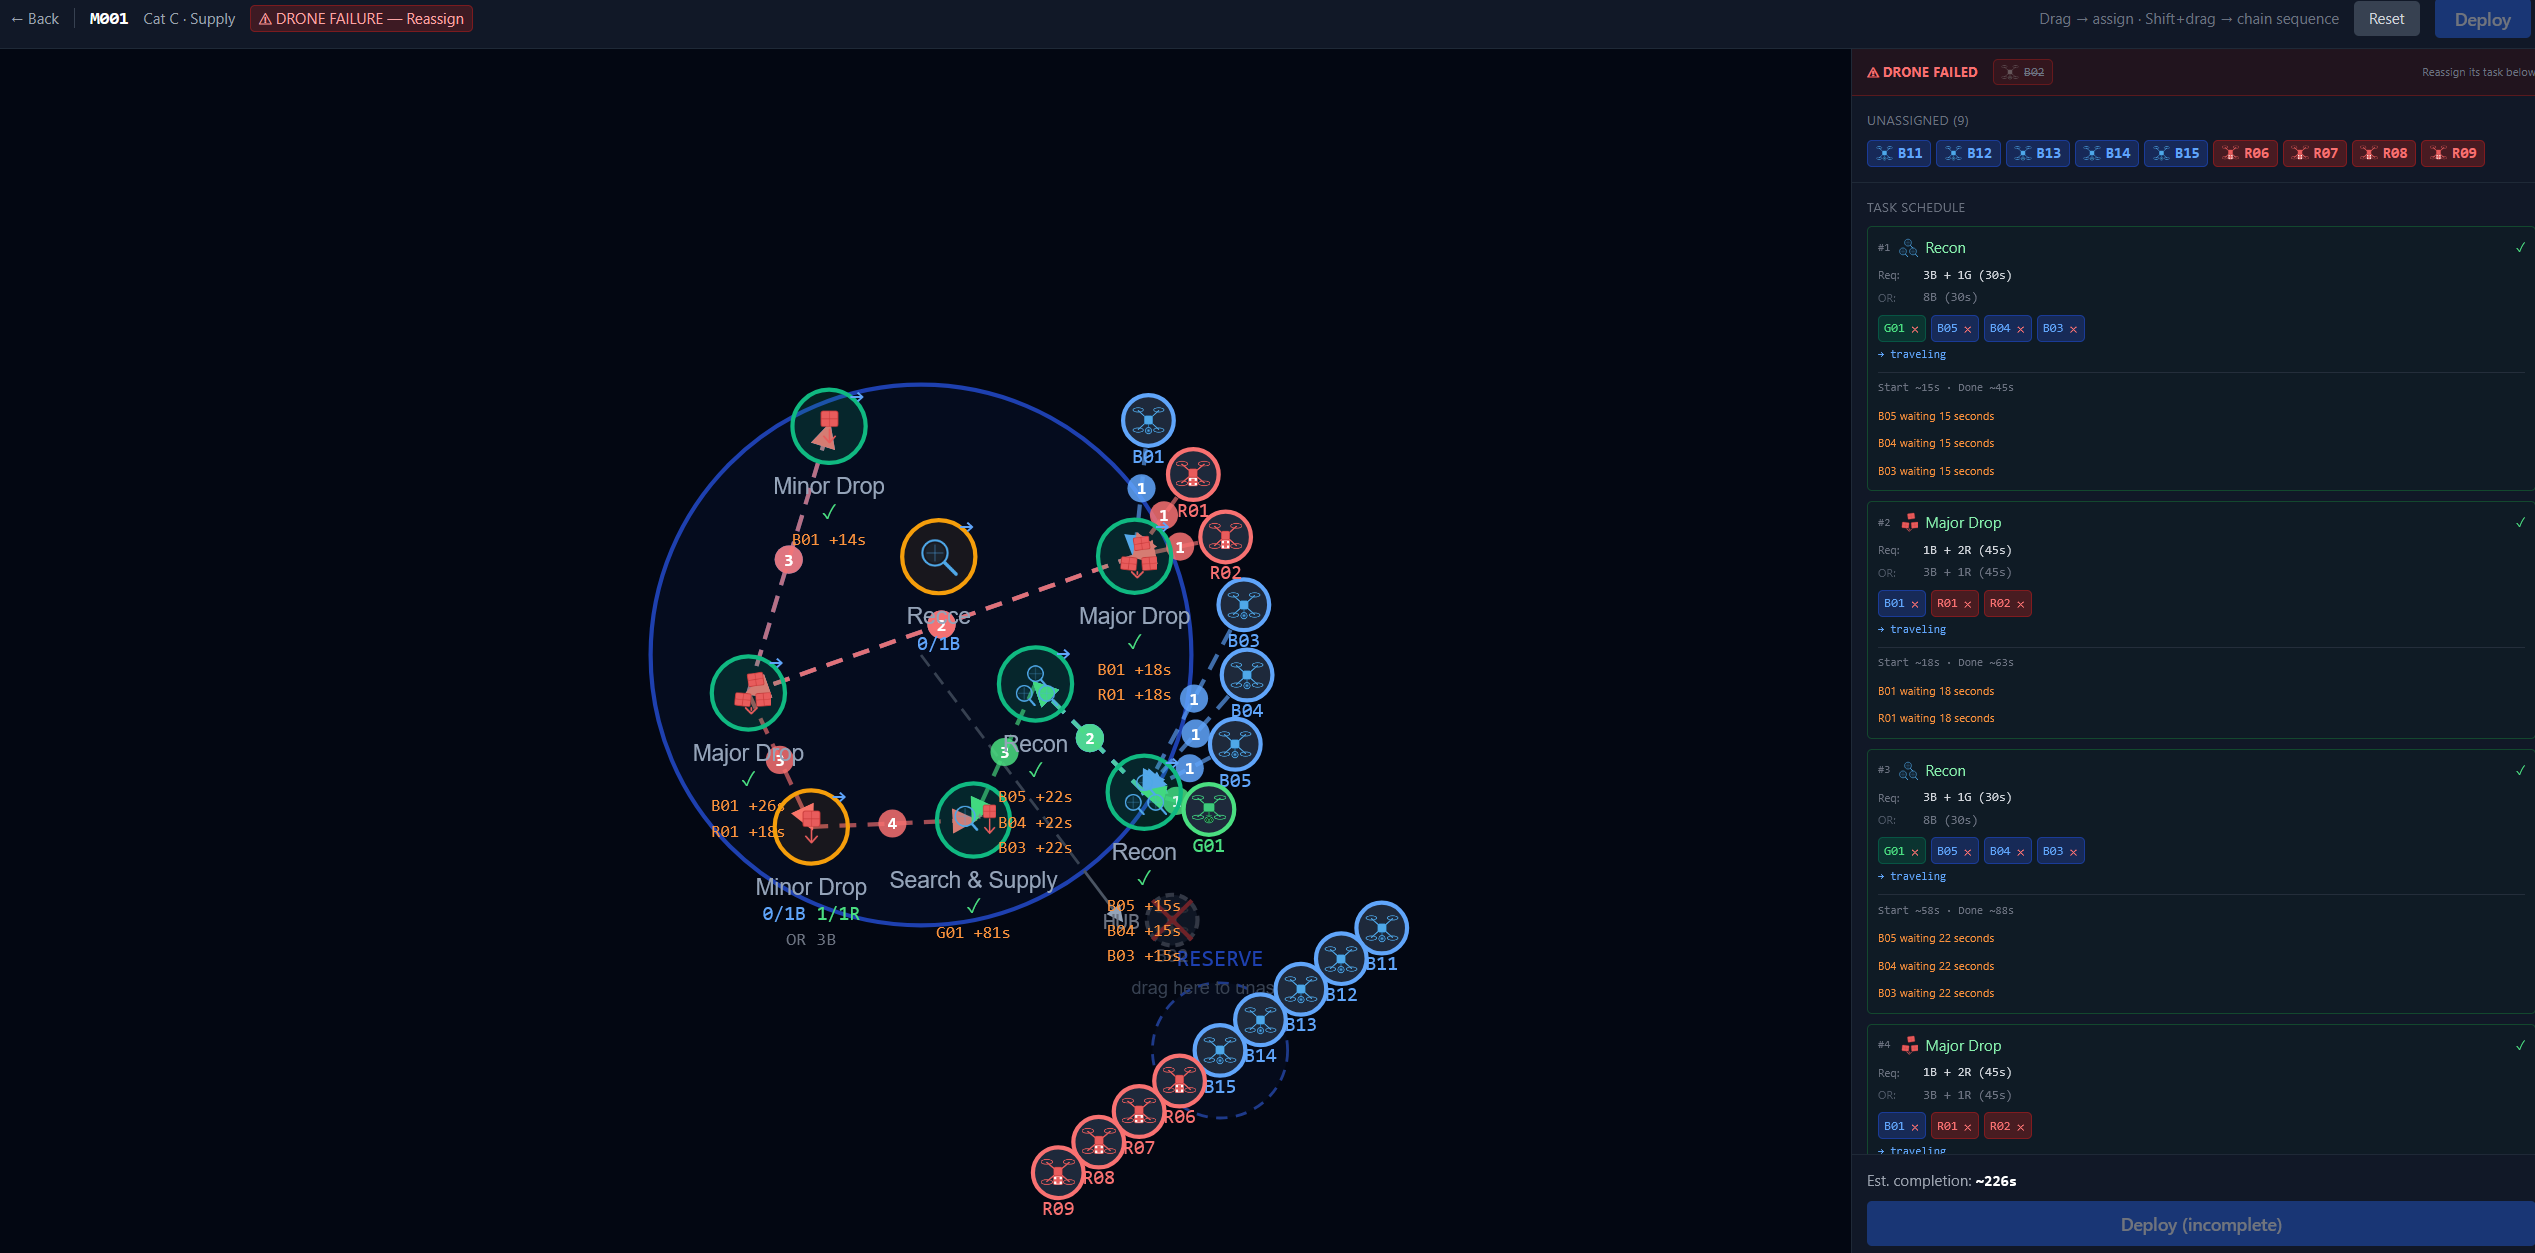
\includegraphics[width=\linewidth]{figs/6}
  \caption{Recovery-mode tactical planner.
           Deployed drones sit at their task-assigned boundary positions; the failed
           drone (greyed, red cross) is shown near the HUB label.
           Reserve drones cluster at the HUB anchor (lower-left) in case the user needs to call additional assets into this mission}
  \label{fig:recovery}
\end{figure}

\section{Proposed Changes}
After meeting Tuesday 19th, the following issues were raised:

\begin{itemize}
    \item Do the two levels of task (strategic and tactical) represent sufficiently different problems? They are both on some level allocation/optimisation problems - is the notion of higher-abstraction for strategic sufficiently different.
    \item Are we likely to sufficiently capture differences between the absence and presence of the agent? What informs people's usage and will they engage with the manual mode in the agent setting?
\end{itemize}

Regarding the first of these, we have considered trying to factor in the increasing level of unpredictability of lower levels as control moves up the abstraction hierarchy. This would require more uncertainty at the tactical level. Some of this is already present, but perhaps more would be useful, although it is difficult to do this without further complicating the study.

Regarding the second, we are considering stressing to the user the importance of failures. Accountability for mistakes might motivate them to allocate manually more often. A ``reliability score'' is assigned to the user and reported to them live. It penalises the user when their allocations fail, and penalises more on tasks that could more easily have been performed. If the user relies on the agent often, more mistakes happen (as the agent sometimes under-allocates etc), and the user is noticeably punished for this. We could test the presence vs absence of this in each condition. Each scenario goes through four 3-minute phases, varying easy and hard allocations at both the strategic and tactical levels, totalling 12 minutes. This gives us data on agent use with or without accountability for its mistakes, and covering difficulty at each scale of the swarm.

% -----------------------------------------------------------------
\section{Experiment Design}\label{sec:studydesign}

\subsection{Design}

The study employs a within-subjects design with two conditions: \textbf{Agent} (Strategic and Tactical Agents available) and \textbf{Manual} (no assistive system). Each participant completes one session per condition. Condition order is counterbalanced across participants to control for learning and fatigue effects.

$N = XX$ participants are recruited from [population].

\subsection{Procedure}

Each study session follows a fixed sequence:
\begin{enumerate}[noitemsep]
  \item \textbf{Pre-study questionnaire.} Demographics, technology comfort, prior experience with autonomous systems, drone operations, or emergency management.
  \item \textbf{Tutorial.} Scripted walkthrough of the interface, asset types, task types, and mission mechanics. In the Agent condition the tutorial additionally covers both assistive tiers. Followed by a free-play practice session of 3 minutes.
  \item \textbf{Trial.} One timed session of duration $T = 10$ minutes, preceded by a one-minute briefing screen.
  \item \textbf{Post-trial survey.} NASA-TLX, trust scale (Agent condition only), and TAM (Agent condition only); see Section~\ref{sec:metrics}.
  \item \textbf{Post-study questionnaire.} Ratings of difficulty and tool usefulness; open-ended reflections on strategy and decision confidence.
\end{enumerate}

The full study (both conditions) lasts approximately 45--60 minutes.

\subsection{Metrics}\label{sec:metrics}

\subsubsection{Objective Performance}

Primary measure: total score $S$ (Equation~\ref{eq:score}). Secondary measures: Green utilisation efficiency; mean mission completion time; reserve depth at allocation events.

\subsubsection{Interaction Behaviour (Agent Condition)}

Every allocation decision in the Agent condition is logged with its situational context: number of active missions, current reserve depth per asset type, incoming mission category, and which action the operator took (Strategic Agent strategy accepted as proposed; accepted after modification; rejected in favour of manual allocation). Tactical Agent posture recommendations are logged alongside whether the operator's subsequent allocation was consistent with the recommended posture. This record supports analysis of \emph{when} operators elect to use the agent and \emph{what advantage} agent-assisted allocations confer relative to counterfactual manual choices.

\subsubsection{Subjective Measures}

After each trial participants complete:
\begin{itemize}[noitemsep]
  \item \textbf{NASA Task Load Index (TLX)}~\cite{hart1988nasa}: six subscales on a 20-point scale; we report the unweighted mean (TLX$_\mu$).
  \item \textbf{Trust in the assistant}~\cite{jian2000foundations} (Agent condition): six items adapted from Jian, Bisantz \& Drury (2000) on a 7-point Likert scale, administered separately for the Strategic and Tactical Agents. Two items (\textit{suspicious}, \textit{wary}) are reverse-scored; a composite trust score is computed as $\frac{\bar{x}_{\mathrm{pos}} - \bar{x}_{\mathrm{neg}} + 6}{12}\times 7$.
  \item \textbf{Technology acceptance (TAM)}~\cite{davis1989perceived} (Agent condition): four items assessing perceived usefulness, ease of use, and intention to use on a 7-point Likert scale; we report the mean (TAM$_\mu$), administered separately for each tier.
\end{itemize}

The post-study questionnaire elicits ratings of difficulty and tool usefulness, and open-ended strategy reflections.

\subsection{Planned Analyses}

RQ1 (performance benefit) is addressed by comparing score $S$, Green utilisation efficiency, and mean mission completion time between Agent and Manual conditions using paired tests. RQ2 (selective use) is examined descriptively: agent engagement rate is modelled as a function of situational covariates (reserve depth, number of active missions, incoming mission category) at the moment of each allocation decision. RQ3 (agent advantage) is estimated by comparing the score contribution of missions allocated with agent assistance against those allocated manually within the Agent condition, controlling for mission category.

% -----------------------------------------------------------------
\section{Results}\label{sec:results}


% -----------------------------------------------------------------
\section{Discussion}\label{sec:discussion}

% -----------------------------------------------------------------
\section{Conclusion}\label{sec:conclusion}


\bibliographystyle{plainnat}
\bibliography{refs}

% -----------------------------------------------------------------
\appendix
\section{Simulation Parameters}\label{app:params}

Table~\ref{tab:params} lists all fixed numerical parameters of the simulation. These values are held constant across all conditions and participants.

\begin{table}[H]
\centering
\caption{Fixed simulation parameters.}
\label{tab:params}
\small
\renewcommand{\arraystretch}{1.3}
\begin{tabular}{llr}
\toprule
\textbf{Parameter} & \textbf{Description} & \textbf{Value} \\
\midrule
\multicolumn{3}{l}{\textit{Asset pool (standard preset)}} \\
Blue drones   & Reconnaissance; speed & 18 units; 9.0\,u/s \\
Red drones    & Aid delivery; speed   & 9 units; 6.0\,u/s  \\
Green drones  & Thermal/specialist; speed & 3 units; 4.2\,u/s \\
\midrule
\multicolumn{3}{l}{\textit{Task execution times and reward weights}} \\
T1 Recce          & 1\,B              & 15\,s;\quad 10\,pts \\
T2 Recon          & 3\,B + 1\,G       & 30\,s;\quad 20\,pts \\
T3 Minor Drop     & 1\,B + 1\,R       & 30\,s;\quad 30\,pts \\
T4 Major Drop     & 1\,B + 2\,R       & 45\,s;\quad 40\,pts \\
T5 Search \& Supply & 1\,R + 1\,G     & 45\,s;\quad 50\,pts \\
\midrule
\multicolumn{3}{l}{\textit{Mission category penalty rates and maximum scores}} \\
A Routine       & & 0.05\,pts/s;\quad 110\,pts \\
B Moderate      & & 0.10\,pts/s;\quad 210\,pts \\
C Significant   & & 0.15\,pts/s;\quad 240\,pts \\
D Critical      & & 0.20\,pts/s;\quad 300\,pts \\
E Mass Casualty & & 0.25\,pts/s;\quad 380\,pts \\
\midrule
\multicolumn{3}{l}{\textit{Session parameters}} \\
Session duration $T$ & Per trial & 10\,min \\
Tutorial free-play   & Practice session & 3\,min \\
Conservative top-up  & Strategic Agent reserve padding & +30\% above minimum \\
Drone failure rate   & Approximate frequency & 1 per session \\
\bottomrule
\end{tabular}
\end{table}

\end{document}